\documentclass[../notes.tex]{subfiles}

\pagestyle{main}
\renewcommand{\chaptermark}[1]{\markboth{\chaptername\ \thechapter\ (#1)}{}}
\setcounter{chapter}{8}

\begin{document}




\chapter{NMR}
\section{NMR Spectroscopy}
\begin{itemize}
    \item \marginnote{2/28:}Announcements.
    \begin{itemize}
        \item Second HW is due Friday at noon.
        \begin{itemize}
            \item We should have everything we need for it after today.
        \end{itemize}
        \item The final will be from 8:00-9:20am on Tuesday.
        \begin{itemize}
            \item It is solely on Anderson's lectures (it's just a second midterm).
            \item Not open note. Shouldn't be too many things to memorize: $g\beta H$, magnetic moment formulas, gnarly stuff like the EXAFS formula we don't need to have memorized.
        \end{itemize}
    \end{itemize}
    \item We now start the lecture.
    \item Relation between EPR and NMR.
    \begin{itemize}
        \item There are many parallels.
        \item NMR is more common than EPR, and much more complicated.
    \end{itemize}
    \item We will start with some simpler NMR examples to build a foundation.
    \item NMR background/underlying principles.
    \begin{itemize}
        \item Like an electron has $S=\pm 1/2$, nuclei also have a given spin $I$.
        \item While a single electron can only be $S=1/2$, a single nucleus can be $I=0,1/2,1,3/2,\dots$.
    \end{itemize}
    \item A few rules about $I$.
    \begin{enumerate}
        \item A nucleus with an odd mass number has a half-integer spin.
        \item A nucleus with an even mass number and an odd atomic number has an integer spin.
        \begin{itemize}
            \item Examples: Deuterium, \ce{{}^14N}, etc.
        \end{itemize}
        \item A nucleus with an even mass number and an even atomic number has zero spin.
    \end{enumerate}
    \item We now investigate the \textbf{Zeeman splitting} of an $I=1/2$ nucleus.
    \begin{itemize}
        \item Like electron spins in EPR, nuclear spins align with or against applied magnetic fields.
        \item The splitting is as in Figure \ref{fig:zeroFieldSplita}.
        \item We know that $\Delta E=\gamma\hbar B_0$, where $\gamma$ is the gyromagnetic ratio and $B_0$ is the applied field.
    \end{itemize}
    \item The notes also consider the $I=1$ case.
    \item \textbf{Zeeman splitting}: The energy difference between a spin aligned with and against a magnetic field.
    \item \textbf{Larmor frequency}: The frequency of electromagnetic radiation that induces a spin flip. \emph{Also known as} \textbf{resonant frequency}. \emph{Denoted by} $\bm{\nu_0}$. \emph{Given by}
    \begin{equation*}
        \nu_0 = \frac{\gamma B_0}{2\pi}
    \end{equation*}
    \begin{itemize}
        \item Takeaway: A nucleus's resonant frequency is determined by $\gamma$ and $B_0$.
    \end{itemize}
    \item Typical values for $B_0$, $\gamma$, and $\nu_0$.
    \begin{itemize}
        \item $B_0$: \SIrange{1.4}{14}{\tesla}.
        \item $\nu_0$: \SIrange{60}{600}{\mega\hertz}, though we can go higher.
    \end{itemize}
    \item Example: The Larmor frequency of some common NMR nuclei under a \SI{9.4}{\tesla} magnet.
    \begin{itemize}
        \item \ce{{}^1H}: We have that
        \begin{equation*}
            \nu_0 = \frac{\gamma B_0}{2\pi}
            = \frac{(\SI{26.8e7}{\per\tesla\per\second})(\SI{9.4}{\tesla})}{2\pi}
            = \SI{4.0e8}{\per\second}
            = \SI{400}{\mega\hertz}
        \end{equation*}
        \item \ce{{}^13C}: \SI{100}{\mega\hertz}.
        \item \ce{{}^31P}: \SI{162}{\mega\hertz}.
        \item \ce{{}^2H}: \SI{61}{\mega\hertz}.
    \end{itemize}
    \item The key limitation of NMR is \emph{sensitivity}.
    \begin{itemize}
        \item The sensitivity for NMR is pretty atrocious. This is because all relevant energies are pretty small (radiofrequency region) and thus hard to detect.
        \item Quantitatively, sensitivity is proportional to the magnetogyric ratio cubed times the number of nuclei (equivalently, the concentration).
        \item This is why MRI is really tough.
        \item Also why you need really big magnets for NMR.
        \item Additional limitation: The signal increases by the square of the applied field strength.
        \begin{itemize}
            \item Limiting by the signal-to-noise ratio; see next lecture.
        \end{itemize}
    \end{itemize}
    \item Aside: Hyperpolarization for NMR.
    \begin{itemize}
        \item Goal: Enhance signal intensity by further polarizing nuclear spins.
        \item Essentially, if you have four particles in the spin ground state and three in the spin excited state, exciting one of the ground state spins won't cause a significantly measurable change. However, if you \emph{hyperpolarize} the system so that there are, for example, six particles in the ground state and only one in the excited state, then inducing an excitation causes a far greater change.
        \begin{itemize}
            \item You can do this with \textbf{dynamic nuclear polarization}, particularly \textbf{triplet DNP}.
            \item Also something akin to ENDOR with Zeeman splitting and microwaves to get a huge polarization buildup. Nobody has pulled this off \emph{in situ} yet, but that's a goal.
        \end{itemize}
        \item There's a scientist in Texas (possibly Christian Hilty??) looking into \textbf{parahydrogen}.
        % \item DNP: Taking a singlet. Photoexciting it with light to generate a triplet. Then intersystem crossing to give you an $M_s$ that is selectively 0. You selectively populate the $M_s=0$ state. If this interacts with your nuclear spin, it causes the polarization; this is \textbf{triplet dynamic nuclear polarization}.
    \end{itemize}
    \item \textbf{Dynamic nuclear polarization}: A technique for hyperpolarization involving the transfer of spin polarization from electrons to nuclei. \emph{Also known as} \textbf{DNP}.
    \item \textbf{Triplet DNP}: Photoexciting a singlet to a triplet and then harnessing intersystem crossing to selectively populate the $M_s=0$ state before transferring this polarization to the nuclei.
    \item \textbf{Parahydrogen}: The spin isomer of hydrogen with the two proton spins aligned antiparallel.
    \item The key advantage of NMR is \emph{resolution}.
    \begin{itemize}
        \item The specific frequency of a given nuclei is often exquisitely sensitive to its chemical environment.
        \item NMR is a Qbit technique: We're using the nuclear spin as a quantum sensor for the system.
        \item This really comes down to shielding.
    \end{itemize}
    \item Shielding.
    \begin{itemize}
        \item A useful (but technically inaccurate) classical analogy.
        \begin{itemize}
            \item If we have an electron and we apply a magnetic field $H_0$ to it in the $z$-direction, our electron will begin to circulate around it and induce a magnetic field in the opposite ($-z$) direction.
            \item The angular frequency $\omega_1$ equals $eH_0/2m_e$.
        \end{itemize}
        \item Takeaway: Applied magnetic fields result in slight changes depending on the nuclear environment.
        \item Because nuclei have very small energy splittings, we can resolve very small energy changes in our NMR spectra; this is the origin of the ppm splitting we're familiar with.
    \end{itemize}
    \item Shielding originates primarily from three places.
    \begin{enumerate}
        \item Nucleus: Specifically how electron-rich or -poor it is.
        \item Solvent: The electrons therein will strongly influence the magnetic field felt by the nuclei.
        \item Chemical environment: Bonds, functional groups, other nuclei, electrons, etc.
    \end{enumerate}
    \item Parts 1 and 3 (electron richness and nuclear factors) are related to each other and are important.
    \begin{itemize}
        \item We usually correct for part 2 using a known solvent shift and an internal standard.
    \end{itemize}
    \item Measuring and describing the \textbf{chemical shift}.
    \begin{itemize}
        \item \SI{1}{\ppm} is a shift in the resonant frequency of a given nucleus. Specifically,
        \begin{equation*}
            \SI{1}{\ppm} = \frac{\nu_1-\nu_\text{ref}}{\nu_0}\times\num{e6}
        \end{equation*}
        \begin{itemize}
            \item $\nu_1$ is the measured Larmor frequency for a given nucleus.
            \item $\nu_\text{ref}$ refers to a single compound that we reference against, e.g., TMS.
            \item $\nu_0$ is the predicted Larmor frequency for said nucleus based on its $\gamma$.
        \end{itemize}
        \item Thus, at \SI{60}{\mega\hertz} (for example), $\SI{1}{\ppm}=\SI{60}{\hertz}$.
        \item Chemical shift lingo.
        \begin{itemize}
            \item More \emph{shielded} nuclei require \emph{higher fields}, have a \emph{lower chemical shift}, and are positioned relatively \emph{upfield}.
            \item More \emph{deshielded} nuclei resonate at \emph{lower fields}, have a \emph{higher chemical shift}, and are positioned relatively \emph{downfield}.
        \end{itemize}
    \end{itemize}
    \item Line widths.
    \begin{itemize}
        \item Recall from EPR: $\tau$ denotes \textbf{lifetime}.
        \item We're limited by the Heisenberg uncertainty principle
        \begin{equation*}
            \Delta E\Delta t = \hbar
            \quad\Longleftrightarrow\quad
            \Delta E = \frac{\hbar}{\tau}
        \end{equation*}
        \item It follows that a long lifetime $\tau$ gives you a small $\Delta E$ and a sharp line.
        \item Typical lifetimes: $\tau_\text{NMR}=\SIrange{1}{100}{\second}$, $\tau_\text{rot}=\SI{e-9}{\second}$, $\tau_\text{vib}=\SI{e-6}{\second}$.
    \end{itemize}
    \item \textbf{Lifetime}: The time that a signal will remain polarized. \emph{Denoted by} $\bm{\tau}$, $\bm{\Delta t}$.
    \item \textbf{Chemical shift}. \emph{Denoted by} $\bm{\sigma}$. \emph{Given by}
    \begin{equation*}
        \sigma = \sigma_d+\sigma_p+\sigma_R+\sigma_e+\sigma_\text{int}
    \end{equation*}
    \begin{itemize}
        \item Each of the five variables represents a contribution to the nucleus from some magnetic component.
        \item $\sigma_d$ is our diamagnetic term.
        \begin{itemize}
            \item Usually positive, so it causes signals to shift downfield.
            \item Most important for \ce{{}^1H} NMR.
            \item Correlates with the $s$-electron density at the nucleus; thus can give us a direct readout of the electron density of the nucleus. Also, more electron rich means more shielded.
        \end{itemize}
        \item $\sigma_p$ is our paramagnetic term.
        \begin{itemize}
            \item Usually negative, so it causes signals to shift upfield.
            \item Most important for heavier elements (e.g., \ce{{}^31P}, \ce{{}^119Sn}, etc.).
            \item A large term in general (larger than $\sigma_d$??).
            \item Distinct usage from paramagnetic \emph{samples} (diamagnetic nuclei can have paramagnetic terms).
        \end{itemize}
        \item $\sigma_R$ is for ring currents.
        \begin{itemize}
            \item Consider a benzene ring for instance. The large induced ring current creates two cones of positive shift and negative regions outside.
            \item Other multiple bonds also contribute in various ways.
            \item For more details, see the discussion associated with Figure \ref{fig:BnzRingCurrent} below.
        \end{itemize}
        \item $\sigma_e$ is for electric fields.
        \item $\sigma_\text{int}$ is for intermolecular effects.
        \item The latter three are often combined into $\sigma_N$.
        \item Recall\dots
        \begin{itemize}
            \item $\sigma>0$ means an upfield shift (lower ppm)
            \item $\sigma<0$ means a downfield shift (higher ppm).
        \end{itemize}
    \end{itemize}
    \item Benzene ring current effects.
    \begin{figure}[h!]
        \centering
        \begin{tikzpicture}
            \fill [blz,opacity=0.5] (0.45,0) arc[start angle=0,end angle=180,x radius=0.45cm,y radius=0.135cm] -- (-1,-2) arc[start angle=180,end angle=0,x radius=1cm,y radius=0.3cm] -- cycle;
            \fill [blz,opacity=0.5] (0.45,0) arc[start angle=0,end angle=-180,x radius=0.45cm,y radius=0.135cm] -- (-1,-2) arc[start angle=-180,end angle=0,x radius=1cm,y radius=0.3cm] -- cycle;
    
            \begin{scope}[yscale=0.3,rotate=-2]
                \node[transform shape]{\chemfig{**6(------)}};
            \end{scope}
    
            \fill [blz,opacity=0.5] (0.45,0) arc[start angle=0,end angle=180,x radius=0.45cm,y radius=0.135cm] -- (-1,2) arc[start angle=180,end angle=0,x radius=1cm,y radius=0.3cm] -- cycle;
            \fill [blz,opacity=0.5] (0.45,0) arc[start angle=0,end angle=-180,x radius=0.45cm,y radius=0.135cm] -- (-1,2) arc[start angle=-180,end angle=0,x radius=1cm,y radius=0.3cm] -- cycle;
    
            \footnotesize
            \node at (0,2) {$+$};
            \node at (0,-2) {$+$};
            \node at (1.3,0) {$-$};
            \node at (-1.3,0) {$-$};
        \end{tikzpicture}
        \caption{The effect of the ring current in benzene.}
        \label{fig:BnzRingCurrent}
    \end{figure}
    \begin{itemize}
        \item It's a fake ring current.
        \item It's a quantum mechanical effect from the interaction of the magnetic field with the degenerate $\pi$ system.
        \item But still, it's a useful classical picture.
        \item Something with Zwitterionic character may be able to give you a "real" ring current.
    \end{itemize}
    \item Most of us have probably seen some of this before. But now we'll move onto something we haven't seen: Heavier nuclei.
    \item With heavier nuclei, $\sigma_p$ dominates.
    \begin{itemize}
        \item The spread is much bigger than with \ce{{}^1H} NMR.
        \item $\sigma_d$ is still there but is typically small and much more constant.
    \end{itemize}
    \item Contributions to $\sigma_p$.
    \begin{itemize}
        \item The orbital angular momentum, largely from the $p,d,f$ orbitals.
        \begin{itemize}
            \item We do \emph{not} consider electron spin here, just orbital spin.
        \end{itemize}
        \item The magnitude of $\sigma_p$ is controlled by mixing.
        \begin{itemize}
            \item Mixing in other states mixes in their angular momentum.
            \item Most common when there is lowered symmetry, low-lying excited states, and lots of EWGs.
            \item Mathematically, we describe $\sigma_p$ with the \textbf{Ramsey equation}.
        \end{itemize}
    \end{itemize}
    \item \textbf{Ramsey equation}: The equation giving the relative magnitude of $\sigma_p$. \emph{Given by}
    \begin{equation*}
        \sigma_p \propto -\left[ \frac{1}{E_\text{es}}-E_\text{gs} \right]\left\langle \frac{1}{r^3} \right\rangle[\pi\text{-bonding term}]
    \end{equation*}
    \begin{itemize}
        \item es denotes the excited state.
        \item gs denotes the ground state.
        \item Rationalizing the energy separation (first) term.
        \begin{itemize}
            \item Alkanes have strong bonds and no low-lying excited states, while alkenes will have lower excited states.
            \item Thus, $\sigma_p$ is greater for alkenes than alkanes, for example.
            \item Takeaway: Unsaturation typically leads to larger paramagnetic terms.
        \end{itemize}
        \item Rationalizing the $1/r^3$ term.
        \begin{itemize}
            \item It is related to how close electrons are to the nucleus.
            \item EWGs decrease electron-electron repulsions, moving electrons closer to the nucleus, thus increasing $\sigma_p$ and shift heavier nuclei more downfield.
        \end{itemize}
        \item The $\pi$-bonding term is complicated; we will not discuss it further.
        \begin{itemize}
            \item It is summed over all relevant interactions.
            \item Depends on the system at hand.
        \end{itemize}
    \end{itemize}
    \item Thus, the chemical shift can provide important chemical information.
    \item However, it can also provide other useful information, such as on \textbf{coupling}.
    \item \textbf{First order system}: A system in which the spread of the nuclei is much higher in ppm than the coupling constant, i.e., in which the following equation is satisfied.
    \begin{equation*}
        \Delta\nu = |\nu_{\ce{A}}-\nu_{\ce{X}}| \gg J_{\ce{AX}}
    \end{equation*}
    \begin{itemize}
        \item $\nu_{\ce{A}}$ is the frequency/ppm shift of nucleus \ce{A}.
        \item $\nu_{\ce{X}}$ is the frequency/ppm shift of nucleus \ce{X}.
        \item $J_{\ce{AX}}$ is the coupling constant between \ce{A} and \ce{X}.
        \item Coupling is relatively simple in first order systems.
        \item We will not get into second order splitting, which occurs when the above inequality is not satisfied and is very complicated.
    \end{itemize}
    \item Example: Consider the following molecule, which has two nuclei of interest (each with $I=1/2$).
    \begin{figure}[H]
        \centering
        \footnotesize
        \chemfig{Cl_3C-C(-[6]Cl)(-[2]{H_A})-C(-[6]Cl)(-[2]{H_X})-Cl}
        \caption{NMR coupling of two neighboring nuclei.}
        \label{fig:couplingTwo}
    \end{figure}
    \begin{itemize}
        \item Comments on the molecule.
        \begin{itemize}
            \item A nasty molecule chemically; would probably destroy the ozone layer and such.
            \item Only two spin-active proton nuclei.
            \item We stick on the \ce{CCl3} group to put the two protons in different chemical environments (gets rid of the reflection plane that would be there if \ce{CCl3} were just \ce{Cl}).
        \end{itemize}
        \item Let's look at the peak structure of \ce{A} first.
        \begin{itemize}
            \item \ce{X} can have one of two values: $M_I=\pm 1/2$.
            \item Thus, \ce{A} can be in two marginally different chemical environments, and hence should appear as a doublet.
        \end{itemize}
        \item The same is true of \ce{X}.
        \item Thus, the full \ce{{}^1H} NMR spectrum should consist of a pair of doublets.
    \end{itemize}
    \item There are two types of coupling.
    \begin{enumerate}
        \item \textbf{Dipolar coupling}. Occurs "through space."
        \begin{figure}[h!]
            \centering
            \begin{subfigure}[b]{0.2\linewidth}
                \centering
                \begin{tikzpicture}
                    \small
                    \node (A)          {\ce{A}};
                    \node (X) at (1,0) {\ce{X}}
                        edge [blx,thick,-stealth] (1,0.7)
                    ;
                    \draw [blx,dashed,->] (1,0.7) to[out=90,in=90,in looseness=3,out looseness=1] (A);
                    \draw [blx,dashed,->] (A) to[out=-90,in=-90,looseness=3] (X);
        
                    \footnotesize
                    \draw [-latex] (-0.5,-0.5) -- node[left]{$B_0$} ++(0,1);
        
                    \path (-1,0) -- (2,0);
                \end{tikzpicture}
                \caption{Opposing.}
                \label{fig:dipolarCouplinga}
            \end{subfigure}
            \begin{subfigure}[b]{0.2\linewidth}
                \centering
                \begin{tikzpicture}
                    \small
                    \node (A)          {\ce{A}};
                    \node (X) at (1,0) {\ce{X}}
                        edge [blx,thick,stealth-] (1,0.7)
                    ;
                    \draw [blx,dashed,<-,shorten <=2pt] (1,0.7) to[out=90,in=90,in looseness=3,out looseness=1] (A);
                    \draw [blx,dashed,<-] (A) to[out=-90,in=-90,looseness=3] (X);
                \end{tikzpicture}
                \caption{Reinforcing.}
                \label{fig:dipolarCouplingb}
            \end{subfigure}
            \caption{Dipolar coupling.}
            \label{fig:dipolarCoupling}
        \end{figure}
        \begin{itemize}
            \item Having a nearby element \ce{X} that is magnetized is like bringing an additional magnet close to \ce{A}, affecting its chemical environment.
            \item \ce{X} can oppose or reinforce the applied magnetic field $B_0$ at \ce{A} (see Figure \ref{fig:dipolarCoupling}).
            \item The field is given by
            \begin{equation*}
                B_{\ce{AX}} = \gamma_{\ce{A}}\gamma_{\ce{X}}\cdot\frac{3\cos^2\theta-1}{r_{\ce{AX}}^2}
            \end{equation*}
            \begin{itemize}
                \item $\gamma$'s are gyromagnetic ratios.
                \item $r_{\ce{AX}}$ is assumed to be big; thus distance is important.
                \begin{itemize}
                    \item Is the exponent a 2 or a 3??
                \end{itemize}
                \item $\theta$ is the angle between the two nuclear spin axes (of \ce{A} and \ce{X}).
                \item What exactly is this field??
            \end{itemize}
            \item Dipolar coupling averages to zero in solution but still affects relaxation.
            \item When \ce{{}^31P} NMR is run, it is done proton decoupled to get bigger shifts.
            \begin{itemize}
                \item How is this relevant??
            \end{itemize}
        \end{itemize}
        \item \textbf{Scalar coupling}. Occurs "through bond."
        \begin{itemize}
            \item Dominates in solution.
            \item We have that
            \begin{equation*}
                E_\text{scalar} = hJM_{I,\ce{A}}M_{I,\ce{X}}
            \end{equation*}
            \item $J$ is our coupling constant in Hertz.
            \item Notes on $J$.
            \begin{itemize}
                \item Can be positive or negative, but in most cases, we don't care what its sign is. We can determine this experimentally if we need it, though.
                \item Proportional to the $s$-character of the bond.
                \item Independent of $H$, so the same on all instruments.
            \end{itemize}
        \end{itemize}
    \end{enumerate}
    \item Dipolar coupling example: The \ce{C3Cl6H2} doublets.
    \begin{figure}[h!]
        \centering
        \begin{tikzpicture}[
            every node/.style=black
        ]
            \small
            \draw (0,3) node[above]{$E$} -- (0,0) -- (6,0) node[right]{$H$};
    
            \footnotesize
            \draw [dashed]
                (1.25,2.3) -- (3,2.3)
                (1.25,0.7) -- (3,0.7)
            ;
    
            \draw [blx,ultra thick]
                (0,1.5) -- ++(0.5,0)
                (1.25,2.3) -- ++(0.5,0)
                (1.25,0.7) -- node[below]{$-\frac{\nu_{\ce{A}}}{2}$} ++(0.5,0)
                (2.5,2.6) -- ++(0.7,0)
                (2.5,2) -- ++(0.7,0)
                (2.5,1) -- ++(0.7,0)
                (2.5,0.4) -- ++(0.7,0)
            ;
            \draw [blx,semithick]
                (0.5,1.5) -- node[above left]{$\beta$} (1.25,2.3)
                (0.5,1.5) -- node[below left]{$\alpha$} (1.25,0.7)
                (1.75,2.3) -- (2.5,2.6)
                (1.75,2.3) -- (2.5,2)
                (1.75,0.7) -- (2.5,1)
                (1.75,0.7) -- (2.5,0.4)
            ;
    
            \node at (3.6,3.1) {\ce{A}};
            \node at (3.6,2.6) {$\beta$};
            \node at (3.6,2) {$\beta$};
            \node at (3.6,1) {$\alpha$};
            \node at (3.6,0.4) {$\alpha$};
    
            \node at (3.9,3.1) {\ce{X}};
            \node at (3.9,2.6) {$\beta$};
            \node at (3.9,2) {$\alpha$};
            \node at (3.9,1) {$\alpha$};
            \node at (3.9,0.4) {$\beta$};
    
            \node at (4.7,3.1) {$M_{I,\ce{A}}$};
            \node at (4.7,2.6) {$-\frac{1}{2}$};
            \node at (4.7,2) {$-\frac{1}{2}$};
            \node at (4.7,1) {$+\frac{1}{2}$};
            \node at (4.7,0.4) {$+\frac{1}{2}$};
    
            \node at (5.7,3.1) {$M_{I,\ce{X}}$};
            \node at (5.7,2.6) {$-\frac{1}{2}$};
            \node at (5.7,2) {$+\frac{1}{2}$};
            \node at (5.7,1) {$+\frac{1}{2}$};
            \node at (5.7,0.4) {$-\frac{1}{2}$};
    
            \draw [rex,thick,stealth-stealth] (2.65,2.3) -- (2.65,2.6);
            \draw [orx,thick,stealth-stealth] (2.85,2) -- (2.85,2.6);
            \draw [ylx,thick,stealth-stealth] (2.65,1) -- (2.65,2);
            \draw [grx,thick,stealth-stealth] (3.05,0.4) -- (3.05,2.6);
        
            \draw [rex,ultra thick] (6.2,2)   -- ++(0.5,0) node[right]{$\frac{J}{4}=JM_{I,\ce{A}}M_{I,\ce{X}}$};
            \draw [orx,ultra thick] (6.2,1.5) -- ++(0.5,0) node[right]{$\frac{J}{2}$};
            \draw [ylx,ultra thick] (6.2,1)   -- ++(0.5,0) node[right]{$\nu_{\ce{A}}-\frac{J}{2}$};
            \draw [grx,ultra thick] (6.2,0.5) -- ++(0.5,0) node[right]{$\nu_{\ce{A}}+\frac{J}{2}$};
    
            \path (-2,0) -- (8,0);
        \end{tikzpicture}
        \caption{Formation of a pair of NMR doublets.}
        \label{fig:NMRpairDoublets}
    \end{figure}
    \begin{itemize}
        \item Analysis of the first splitting (originates from the applied magnetic field).
        \begin{itemize}
            \item Of the left two connecting lines, the lower one is referred to as the \textbf{$\bm{\alpha}$-manifold} and the upper one is referred to as the \textbf{$\bm{\beta}$-manifold}.
            \begin{itemize}
                \item What exactly are these?? Relation to $\alpha,\beta$ designation of spin from \textcite{bib:CHEM26100Notes}.
            \end{itemize}
            \item The energy of the upper state at the end of the $\beta$-manifold is given by
            \begin{equation*}
                E = -\frac{\gamma}{2\pi}B_0(1-\sigma_{\ce{A}})M_{I,\ce{A}}
                = -\nu_{\ce{A}}M_{I,\ce{A}}
                = \frac{\nu_{\ce{A}}}{2}
            \end{equation*}
            \begin{itemize}
                \item There is a sign flip in the last equality because $M_{I,\ce{A}}$ is negative.
            \end{itemize}
            \item Per the definitions of the green and yellow gaps in Figure \ref{fig:NMRpairDoublets}, the energy difference between the two states at the end of the $\alpha$- and $\beta$-manifolds will just be $\nu_{\ce{A}}$.
            \item Takeaway: In the absence of coupling, one peak corresponds to \ce{A} at the frequency $\nu_{\ce{A}}$.
        \end{itemize}
        \item We now factor in the second splitting (originates from coupling).
        \begin{itemize}
            \item We label the resultant states with a second set of $\beta$'s and $\alpha$'s.
            \begin{itemize}
                \item The signs are related to the signs of the fields from the other nucleus.
            \end{itemize}
            % \item $JM_{I,\ce{A}}M_{I,\ce{X}}=J/4$ is the secondary splitting.
            % \begin{itemize}
            %     \item Thus, $J/2$ is the energy difference between $\beta\beta$ and $\beta\alpha$.
            % \end{itemize}
            % \item Similarly\dots
            % \begin{itemize}
            %     \item $\nu_{\ce{A}}-J/2$ is the energy difference between $\beta\alpha$ and $\alpha\alpha$.
            %     \item $\nu_{\ce{A}}+J/2$ is the energy difference between $\alpha\beta$ and $\beta\beta$.
            % \end{itemize}
            \item Selection rule: $\Delta M_I=\pm 1$.
            \begin{itemize}
                \item Thus, only $\alpha\alpha\to\beta\alpha$ (yellow) and $\alpha\beta\to\beta\beta$ (green) are allowed.
            \end{itemize}
            \item From the frequencies of these two transitions, the splitting in the doublet is
            \begin{equation*}
                J = \left( \nu_{\ce{A}}+\frac{J}{2} \right)-\left( \nu_{\ce{A}}-\frac{J}{2} \right)
            \end{equation*}
            \item $J$ is typically small compared to $\nu_{\ce{A}}$.
            \item Takeaway: Factoring in coupling, we will observe a \emph{doublet} centered around $\nu_{\ce{A}}$. However, $\nu_{\ce{A}}$ is no longer an allowable transition; only the yellow and green ones are (note that these are centered around $\nu_{\ce{A}}$). The peaks corresponding to the yellow and green transitions will be separated by $J$, as described above.
        \end{itemize}
    \end{itemize}
    \item Scalar coupling example: A diatomic molecule.
    \begin{figure}[H]
        \centering
        \begin{tikzpicture}
            \footnotesize
            \node [circle,draw=rex] (A) {A}
                edge [blx,thick,-stealth,shorten <=1mm] (0,0.8)
            ;
            \node [circle,draw=rex] (X) at (1.5,0) {X}
                edge [rex] node[above]{${\color{blx}\downharpoonleft\hspace{-1pt}\upharpoonright}$} (A)
                edge [blx,thick,stealth-,shorten <=1mm] (1.5,0.8)
            ;
        \end{tikzpicture}
        \caption{Scalar coupling in a diatomic molecule.}
        \label{fig:scalarCouplingDiatomic}
    \end{figure}
    \begin{itemize}
        \item How scalar coupling works in more detail (very complicated, but a nice simplistic picture).
        \begin{itemize}
            \item Empirical observation: Electrons and nuclei prefer to align antiparallel.
            \item Notice how each nucleus in Figure \ref{fig:scalarCouplingDiatomic} is aligned antiparallel to the nearest electron.
            \item Naturally, the electrons are also aligned antiparallel since they are in the same bonding orbital.
            \item Thus, the neighboring nuclei prefer to be anti-parallel because of the indirect interaction chain of nucleus-electron, electron-electron, electron-nucleus.
        \end{itemize}
        \item At this point, some of our previous observations should make more sense.
        \begin{itemize}
            \item Example: Scalar coupling scales with $s$-character because greater $s$-character maximizes electron-nucleus interactions.
        \end{itemize}
        % \item As \ce{A} is polarized, there will be some coupling constant to \ce{X}.
        % \item As our nuclear spins (big arrows) point one direction, they polarize the bonding electrons in the other direction.
        % \item Takeaway: Neighboring spins will be antiparallel.
        \item We have no way of measuring the sign of $J$ in an NMR experiment. In order to do the transition, we can see why $s$-character matters: The more the electrons interact with the nucleus (higher $s$-character means closer to nuclei), the stronger the effect will be.
        \begin{itemize}
            \item What is the effect?? What is scalar coupling? How does it show up? How do all of the equations fit together?
        \end{itemize}
        \item On the sign of $J$ for neighboring nuclei.
        \begin{itemize}
            \item If we have a single bond, then $J>0$ and antiparallel spins are more stable.
            \item If we have a double bond, then $J<0$ and parallel spins are more stable.
            \item In general, an odd number of bonds means $J>0$ and an even number of bonds means $J<0$.
            \begin{itemize}
                \item There are many exceptions, though.
            \end{itemize}
        \end{itemize}
        \item On the magnitude of $J$.
        \begin{itemize}
            \item 2-bond: ${}^2J_{\ce{HH}}=\SIrange{10}{25}{\hertz}$. Are these values negative?? $sp^2$ can be $+\SI{41}{\hertz}$.
            \item 3-bond: ${}^3J_{\ce{HH}}=\SIrange{0}{25}{\hertz}$.
        \end{itemize}
    \end{itemize}
    \item Coupling constants and electronic proximity to the nucleus.
    \begin{table}[h!]
        \centering
        \small
        \renewcommand{\arraystretch}{1.2}
        \begin{tabular}{ccc|ccc}
            \textbf{Compound} & \textbf{Hybridization} & \textbf{$\bm{J_\textbf{CH}}$ (Hz)} & \textbf{EWG} & $\bm{\chi}$ & \textbf{$\bm{J_\textbf{CH}}$ (Hz)}\\
            \hline
            Ethane    & $sp^3$ & 125 & \ce{CH3-F}         & 4.0  & 150\\
            Ethene    & $sp^2$ & 156 & \ce{CH3-Cl}        & 3.2  & 150\\
            Benzene   & $sp^2$ & 159 & \ce{CH3-OH}        & 3.4  & 141\\
            Cubane    &        & 160 & \ce{CH4}           & 2.2  & 125\\
            Acetylene & $sp$   & 248 & \ce{Cp2Zr(CH3)(I)} & 1.3  & 120\\
            \ce{H-H}  & $s$    & 284 & \ce{CH3-Li}        & 0.98 & 98\\
        \end{tabular}
        \caption{Coupling constants and molecular electronics.}
        \label{tab:couplingElectron}
    \end{table}
    \begin{itemize}
        \item The last coupling constant on the left is technically a $J_{\ce{HH}}$, not a $J_{\ce{CH}}$.
        \item The left exhibits the expected trend based on $s$-character: Compounds that maximize $s$-character and place electrons closer to the nucleus have higher coupling constants.
        \item The right exhibits the expected trend based on \textbf{Bent's rule}: Compounds with less electronegative EWGs must give more $s$-character to bonding; thus, there is less $s$-character to promote (scalar) coupling and the coupling constant diminishes.
        \item You can quantitatively derive this stuff with MO theory.
        \item Observing these coupling constants: They show up under \ce{{}^13C} NMR that isn't proton decoupled.
    \end{itemize}
    \item \textbf{Bent's rule}: More electronegative elements prefer $p$-character.
    \begin{itemize}
        \item See \textcite{bib:CHEM20100Notes} for more.
    \end{itemize}
    \item Aside: Diamond vacancy centers in quantum computing.
    \begin{itemize}
        \item One of the first things used for a quantum computer was an NMR.
        \item The first quantum computation was performed via NMR spectroscopy.
        \item It was a funky molecule, just enough stuff to do quantum computation, but it worked.
    \end{itemize}
    \item A couple more notes about coupling constants.
    \begin{figure}[h!]
        \centering
        \footnotesize
        \begin{subfigure}[b]{0.3\linewidth}
            \centering
            \chemfig{M(-@{P1}PR_3)(-[2]@{P2}PR_3)(-[4]R_3@{P3}P)(-[6,,,,black!20]{\color{black!20}P}|{\color{black!20}R_3})}
            \chemmove{
                \draw [rex,thick,-,shorten <=3pt,shorten >=12pt] (P1) to[out=90,in=0,looseness=1.2] node[above right,black]{$J_\textit{cis}$} (P2);
                \draw [rex,thick,-,shorten <=3pt,shorten >=3pt] (P1) to[out=-90,in=-90,looseness=1.5] node[pos=0.25,below right,black]{$J_\textit{trans}$} (P3);
            }
            \caption{\emph{cis} vs. \emph{trans}.}
            \label{fig:couplingSpecialCasea}
        \end{subfigure}
        \begin{subfigure}[b]{0.3\linewidth}
            \centering
            \chemfig{(-[:120]H)--[:60]H}
            \hspace{2em}
            \begin{tikzpicture}
                \draw circle (4mm);
    
                \draw (90:0.4) -- (90:0.6) node(H1)[above]{\ce{H}};
                \draw (30:0.4) -- (30:0.6) node(H2)[above right,yshift=-2pt]{\ce{H}};
    
                \draw [rex,thick] (H1) to[out=0,in=130] node[above right,black]{$\theta$} (H2);
            \end{tikzpicture}
            \caption{Viscinal hydrogens.}
            \label{fig:couplingSpecialCaseb}
        \end{subfigure}
        \begin{subfigure}[b]{0.3\linewidth}
            \centering
            \chemfig{@{HB}{H_B}-[:30](=[2](-[:150]@{HA}{H_A})(-[:30,,,,black!20]\textcolor{black!20}{Cl}))-[:-30]@{HC}{H_C}}
            \chemmove{
                \draw [rex,thick,-,shorten >=3pt] (HA) to[bend left=60,looseness=1.3] node[pos=0.75,above right,black]{$J_{AC}$} (HC);
                \draw [rex,thick,-,shorten <=1pt,shorten >=1pt] (HB) to[bend right=30] node[below,black]{$J_{BC}$} (HC);
                \draw [rex,thick,-,shorten <=1pt,shorten >=3pt] (HA) to[bend right=30] node[left,black]{$J_{AB}$} (HB);
            }
            \vspace{2em}
            \caption{Olefins.}
            \label{fig:couplingSpecialCasec}
        \end{subfigure}
        \caption{Special cases in coupling.}
        \label{fig:couplingSpecialCase}
    \end{figure}
    \begin{enumerate}
        \item \emph{cis} vs. \emph{trans} metal complexes.
        \begin{itemize}
            \item $J_\textit{trans}>J_\textit{cis}$.
            \item Example: If we have a square planar coordination compound with four phosphenes, the two pairs of \emph{trans} ligands will (independently) couple more than any of the four pairs of \emph{cis} ligands.
            \item Why: Same argument as \emph{trans} effect; make an MO argument that \emph{trans} will overlap better.
        \end{itemize}
        \item Viscinal coupling: Coupling of atoms separated by two other atoms.
        \begin{itemize}
            \item Example: Two hydrogens on different carbons of ethane.
            \item Coupling magnitude: Depends on the dihedral angle $\theta$ from the Newman projection.
            \item For syn and anti conformers, $J$ will be larger.
            \item For gauche conformers, $J$ will be smaller.
        \end{itemize}
        \item Olefins.
        \begin{itemize}
            \item Example: Vinyl chloride.
            \item $J_{\ce{AC}}=\SIrange{12}{18}{\hertz}$. Sometimes referred to as \emph{trans}.
            \item $J_{\ce{BC}}=\SIrange{0}{3}{\hertz}$. Sometimes referred to as \emph{gem}.
            \item $J_{\ce{AB}}=\SIrange{6}{12}{\hertz}$. Sometimes referred to as \emph{cis}.
        \end{itemize}
    \end{enumerate}
    \item A more realistic view of spins under a magnetic field.
    \begin{itemize}
        \item We may treat the collection of polarized molecules as an ensemble of spins in space.
        \item However, just because a magnetic field has been applied doesn't mean that each nuclear spin is perfectly poised along the $z$-axis.
        \item Rather, there are still residual $x$- and $y$-components that will precess around the $z$-axis.
        \begin{itemize}
            \item We have, in fact, a whole distribution of spins which are arranged in some cone around the $z$-axis. We do indeed have a random and equally dispersed $x,y$-spins.
            \item The precession is called a \textbf{Larmor precession} and occurs at the \textbf{Larmor frequency}.
        \end{itemize}
        % \item Let's capture the fraction of proton spins that are aligned in the $z$-direction.
        % \item These spins are not static; they're precessing about the $z$-axis.
        % \item The precession $\nu_0=-\gamma B_0/2\pi$ is the \textbf{Larmor frequency}.
    \end{itemize}
    \item The NMR experiment.
    \begin{itemize}
        \item What we do is take the ensemble of spins and apply a \ang{90} radiofrequency pulse to project the net magnetization onto the $x$-axis. Then, we monitor the precession rate about the $xy$-plane.
        \item This is called a \textbf{Hahn echo experiment}.
        \begin{itemize}
            \item We also use this technique in pulsed EPR experiments.
        \end{itemize}
        \item We then Fourier transform the wave to get it back to normal.
        \item Misc. notes.
        \begin{itemize}
            \item The $x$- and $y$-components vary in time.
            \item Both $\alpha$ and $\beta$ (up and down) spins precess at the same frequency.
            \item Chemically equivalent nuclei precess at the same frequency, but are not necessarily in phase.
            \item While the $x$- and $y$-components are scattered, there is still net polarization along $z$ and hence a net magnetization in this direction.
        \end{itemize}
    \end{itemize}
    \item Next time.
    \begin{itemize}
        \item Wikipedia description of the Hahn Echo experiment (really good).
        \item A bit more on NMR, too, to be wrapped up at the beginning of the lecture.
    \end{itemize}
\end{itemize}



\section{NMR Wrap-Up and Examples from the Literature}
\begin{itemize}
    \item \marginnote{3/2:}HW extended until Friday at \emph{midnight}.
    \item Today: Finish up NMR and then some examples. We'll finish about 15 mins early, most likely.
    \item We begin today by discussing \textbf{spin-spin relaxation}, the time constant of which is denoted by $T_2$.
    \begin{itemize}
        \item See Lecture 7.1 on EPR for more.
    \end{itemize}
    \item Recall that under the influence of a magnetic field applied along the $z$-axis, the spins align along $H_z$.
    \item \textbf{$\bm{90^\circ}$ radiofrequency pulse}: A pulse of electromagnetic radiation in the radiofrequency region, the intensity and time of which is calibrated to rotates all Larmor precessions by \ang{90} so as to align them along the $x$-axis.
    \begin{figure}[h!]
        \centering
        \begin{tikzpicture}[
            every node/.style=black
        ]
            \footnotesize
            \begin{scope}
                \draw [-stealth] (0,0,0) -- (1.5,0,0) node[right]{$x$};
                \draw [-stealth] (0,0,0) -- (0,0,1.5) node[below left]{$y$};
                \draw [-stealth] (0,0,0) -- (0,1.5,0) node[above]{$z$};
    
                \draw [grx,thick,-latex] (0,0,0) -- (0,1.2,0) node[above right,yshift=-2mm]{$B_0$};
    
                \draw [blx,very thick,-latex] (0,0,0) -- (0,0.8,0);
                \draw [bly,dashed] plot[domain=0:360] ({0.8*cos(\x)},0.6,{0.8*sin(\x)});
                \foreach \x in {-30,-70,-105,-135,-200} {
                    \draw [bly,semithick,-latex] (0,0,0) -- ({0.8*cos(\x)},0.6,{0.8*sin(\x)});
                }
            \end{scope}
            \draw [ultra thick,-latex] (2.5,0) -- node[above]{\ang{90}} node[below]{RF} ++(1,0);
            \begin{scope}[xshift=5cm]
                \draw [-stealth] (0,0,0) -- (1.5,0,0) node[right]{$x$};
                \draw [-stealth] (0,0,0) -- (0,0,1.5) node[below left]{$y$};
                \draw [-stealth] (0,0,0) -- (0,1.5,0) node[above]{$z$};
    
                \draw [blx,very thick,-latex] (0,0,0) -- (0.8,0,0);
            \end{scope}
            \draw [ultra thick,-latex] (7.5,0) -- node[above]{$t$} ++(1,0);
            \begin{scope}[xshift=10cm]
                \draw [-stealth] (0,0,0) -- (1.5,0,0) node[right]{$x$};
                \draw [-stealth] (0,0,0) -- (0,0,1.5) node[below left]{$y$};
                \draw [-stealth] (0,0,0) -- (0,1.5,0) node[above]{$z$};
    
                \draw [blx,very thick,-latex] (0,0,0) -- (0.5,0,0);
                \draw [bly,dashed] plot[domain=0:360] ({0.8*cos(\x)},0.0,{0.8*sin(\x)});
                \foreach \x in {65,40,-40,-85} {
                    \draw [bly,semithick,-latex] (0,0,0) -- ({0.8*cos(\x)},0,{0.8*sin(\x)});
                }
            \end{scope}
        \end{tikzpicture}
        \caption{A \ang{90} pulse.}
        \label{fig:90Pulse}
    \end{figure}
    \begin{itemize}
        \item Once there, the precessions continue about the applied magnetic field and return to $z$-equilibrium.
        \item Decoherence occurs because the spins that are offset in phase spread out.
        \begin{itemize}
            \item We can watch the frequency of this with respect to time to learn the precession frequencies for each proton.
        \end{itemize}
        \item At $5T_2$'s, we'll have about 99.3\% decay.
        \begin{itemize}
            \item $T_2$ is on the order of seconds.
        \end{itemize}
        \item See \textcite{bib:CHEM26700Notes} for more.
    \end{itemize}
    \item \textbf{Hahn echo experiment}: A \ang{90} pulse, followed by decoherence, followed by a \ang{180} pulse, followed by recoherence. \emph{Also known as} \textbf{HE}, \textbf{spin echo experiment}.
    \begin{itemize}
        \item The echo: After the \ang{180} pulse, things feel the opposite field, so the ones that are slow speed up and the ones that are fast slow down. This is what results in decoherence.
        \item See the GIF on Wikipedia (\href{https://en.wikipedia.org/wiki/Spin_echo}{link}).
        \item We can measure the decoherence time using such an experiment.
        \begin{itemize}
            \item In particular, the intensity of the echo relative to the initial signal is proportional to
            \begin{equation*}
                \e[-2t/T_2]
            \end{equation*}
            \item Rigorously, we derive the above result from the rate law.
            \begin{align*}
                \dv{M_y'}{t} &= -\frac{M_y'}{T_2}\\
                M_y' &= M_0\e[-t/T_2]
            \end{align*}
            \item $T_2$ is equal to half the time until the echo. $T_1$ is related to the magnitude of the echo because that will tell us what proportion of the magnetization has gone back to the $z$-axis??
        \end{itemize}
    \end{itemize}
    \item The other decay is \textbf{spin-lattice} ($T_1$).
    \begin{itemize}
        \item We put the spin on the $y$-axis, making the $z$-component zero.
        \item Then it slowly grows back.
        \item Rate law.
        \begin{align*}
            \dv{M_0-M_z}{t} &= \frac{M_0-M_z}{T_1}\\
            M_z &= M_0[1-\e[-t/T_1]]
        \end{align*}
    \end{itemize}
    \item Both $T_1$ and $T_2$ happen simultaneously, but $T_1>T_2$.
    \item Signal-to-noise ($S/N$) ratio:
    \begin{equation*}
        S/N \propto \sqrt{n}
    \end{equation*}
    \begin{itemize}
        \item $n$ is the number of scans.
        \item The moral of the story is make your samples concentrated so you can use fewer scans.
    \end{itemize}
    \item Nuclear Overhauser Effect (NOE): Decoupling.
    \begin{equation*}
        \eta_{\ce{A}(X)} = \frac{I_{\ce{A}}\mu_{a\ce{X}}-I_{\ce{X}}}{I_{\ce{X}}} = \frac{\gamma_{\ce{X}}}{2\gamma_{\ce{A}}}
    \end{equation*}
    \begin{itemize}
        \item Basic idea behind decoupling/the NOE: Blasting your sample with magnetism in the $x$-direction to constantly flip the spins and saturate them. Essentially, we saturate a given frequency or transition with rf radiation.
        \begin{itemize}
            \item Do I have this right??
        \end{itemize}
        \item Decoupling can increase or decrease the intensity of a given nuclear signal.
        \item By the above equation, the NOE depends on the sign and the magnitude of the gyromagnetic ratios of the two elements, where we are taking the spectrum of \ce{A} with \ce{X} decoupled.
        \item We sum this over all different nuclei that are contributing.
        \item We denote a spectrum that's been proton-decoupled with squiggly brackets, e.g., \ce{{}^13C}\{\ce{{}^1H}\} denotes a proton-decoupled \ce{{}^13C} NMR experiment.
        \item Dipole relaxation.
        \begin{equation*}
            R_{1DDA(X)} \propto r_{\ce{AX}}^6
        \end{equation*}
        \begin{itemize}
            \item We expect a large NOE when \ce{A} and \ce{X} are close, and \ce{A} relaxes primarily by dipole-dipole (DD) from \ce{X}.
        \end{itemize}
        \item Example: Consider the following olefin.
        \begin{figure}[H]
            \centering
            \footnotesize
            \begin{subfigure}[b]{0.3\linewidth}
                \centering
                \chemfig{HO_2C-[:30](-[:-30]CH_3)=[2](-[:150]HO_2C)(-[:30]H)}
                \caption{\emph{cis} protons.}
                \label{fig:NOEcisTransa}
            \end{subfigure}
            \begin{subfigure}[b]{0.3\linewidth}
                \centering
                \chemfig{H_3C-[:30](-[:-30]CO_2H)=[2](-[:150]HO_2C)(-[:30]H)}
                \caption{\emph{trans} protons.}
                \label{fig:NOEcisTransb}
            \end{subfigure}
            \caption{Determining olefin stereochemistry with the Nuclear Overhauser Effect.}
            \label{fig:NOEcisTrans}
        \end{figure}
        \begin{itemize}
            \item The resultant NOEs are
            \begin{align*}
                \eta_\textit{cis} &= 0.29&
                \eta_\textit{trans} &= 0.06
            \end{align*}
            \item If the methyl protons and lone proton are \emph{cis} to each other, we'll see a large NOE.
            \item Barely any NOE for the \emph{trans} case.
        \end{itemize}
        \item This is a good NOESY way to determine if a compound is \emph{cis} vs \emph{trans}.
        \begin{itemize}
            \item Technically, this is a simplistic treatment and we would need to consider all relaxation pathways in reality.
            \item NOE only measures the contribution from DD relaxation.
            \item What does the acronym NOESY mean??
        \end{itemize}
    \end{itemize}
    \item Aside: Acronyms in NMR.
    \begin{itemize}
        \item Only works for diamagnetic compounds, but it's ok.
        \item There's a lot of nasty acronyms in NMR (that's just a thing), but if we ever want to do any of them, Josh in the NMR facility knows how they're preprogrammed into our spectrometers.
    \end{itemize}
    \item Last kind of experiment we're interested in: DEPT.
    \item Distortionless enhancement by polarization transfer (DEPT).
    \begin{figure}[h!]
        \centering
        \begin{tikzpicture}[
            every node/.style=black
        ]
            \footnotesize
            \draw [grx,thick] (0,1.5) node[left]{\ce{{}^1H}}
                -- ++(2,0)
                -- ++(0,0.5)
                -- node[below]{\ang{90}} ++(0.6,0)
                -- ++(0,-0.5)
                -- node[above]{$\frac{1}{2}J$} ++(2,0)
                -- ++(0,0.5)
                -- node[below]{\ang{180}} ++(1.2,0)
                -- ++(0,-0.5)
                -- node[above]{$\frac{1}{2}J$} ++(2,0)
                -- ++(0,0.5)
                -- node[below]{$\theta\pm y$} ++(1,0)
                -- ++(0,-0.5)
                -- node[above]{$\frac{1}{2}J$} ++(2,0)
                -- ++(0,0.5)
                -- node[below]{\{\ce{{}^1H}\}} ++(1,0)
                -- ++(0,-0.5)
            ;
            \draw [grx,thick] (0,0) node[left]{\ce{{}^13C}}
                -- ++(5.2,0)
                -- ++(0,0.5)
                -- node[below]{\ang{90}} ++(0.6,0)
                -- ++(0,-0.5)
                -- node[above]{$\frac{1}{2}J$} ++(2,0)
                -- ++(0,0.5)
                -- node[below]{\ang{180}} ++(1.2,0)
                -- ++(0,-0.5)
                -- node[above]{$\frac{1}{2}J$} ++(2,0)
                -- node[right]{Acquisition} ++(0,0.5)
            ;
    
            \draw [decorate,decoration=brace] (2,2.5) -- node[above=1mm]{\ce{H} spin echo} ++(5.8,0);
            \draw [decorate,decoration={brace,mirror}] (5.2,-0.5) -- node[below=1mm]{\ce{C} spin echo} ++(5.8,0);
        \end{tikzpicture}
        \caption{Pulse sequence in a DEPT experiment.}
        \label{fig:DEPTpulses}
    \end{figure}
    \begin{itemize}
        \item This method allows for information on the multiplicity, e.g., of hydrogens on carbons.
        \item This is between a proton and another nucleus, unlike NOESY which was between two protons.
        \item Notes on the method.
        \begin{itemize}
            \item We do a Hahn echo for both the proton and carbon.
            \item We'll end up with positive and negative peaks corresponding to the number of attached methyls.
            \item The last thing for carbon is acquisition. We measure by varying $y$.
        \end{itemize}
    \end{itemize}
    \item This concludes NMR.
    \begin{itemize}
        \item Do we need to know anything about the rest of the experiments in the notes??
    \end{itemize}
    \item We now look through some literature examples.
    \item \textcite{bib:MossbauerSpectrum}.
    \begin{itemize}
        \item First example: A beautiful Mossbauer spectrum.
    \end{itemize}
    \item \textcite{bib:RittleP450}.
    \begin{itemize}
        \item P450 is kind of the blow-torch of the cell; breaks things down.
        \item Jon Rittle is now a professor at Berkeley, but he was an undergrad at Penn State when he published this pretty seminal paper.
        \item Anderson worked with Rittle in a glovebox for many years, which is why he knows so much of this story.
        \item First up: UV-Vis. One of the hallmarks is green color, and Rittle found this and was very excited.
        \item Mossbauer: At \SI{4}{\kelvin}, you get magnetic splitting.
        \item EPR: Gives more info on where an electron is in an enzymatic environment.
    \end{itemize}
    \item \textcite{bib:Coord7EXAFS}.
    \begin{itemize}
        \item They do a lot of EXAFS fitting, and eventually find that the best fit is a sevenfold coordination model.
    \end{itemize}
    \item \textcite{bib:AndersonPhD}.
    \begin{itemize}
        \item Anderson's PhD work.
        \item Used a whole bunch of techniques to pin down the identity of their compound.
    \end{itemize}
    \item \textcite{bib:EDelocal}.
    \begin{itemize}
        \item Electron is fully delocalized.
    \end{itemize}
    \item That's it.
    \item Do we have to know anything about the examples for the final, or was that just for our own enrichment?
    \item PSet 2 questions.
    \item Question 1: Did you mean to put the \ce{N-H} stretching frequencies in the 3000's?
    \begin{itemize}
        \item These are likely bending modes.
        \item \ce{NH2} can have a symmetric and asymmetric bending mode.
    \end{itemize}
    \item Question 2.
    \begin{figure}[H]
        \centering
        \footnotesize
        \chemfig{-?[1]-[:60]O-Cu?[2]-O-[:-60](-)-[:-120]O-[4]Cu?[2,,dashed]-[4]O?[1]}
        \caption{Copper (II) acetate structure.}
        \label{fig:CuOAcStruct}
    \end{figure}
    \begin{itemize}
        \item We \emph{could} draw out the whole splitting of one copper followed by splitting of another copper, but it will be easier if we just add the contributions of the two coppers and split once.
        \item Essentially, we use the $2nI+1$ rule to get 7 lines. Then we sum the $M_I$'s of the two copper nuclei and split over $-3,-2,\dots,3$ for our fine splitting after we've originally Zeeman split the electron spin. This gives us the number of lines. For intensity, think about how many \emph{microstates} can add to $-3$, $-2$, etc.
        \item This intensity rule is allowed. That's what our EPR spectrum is telling us, that it's ok to sum the contributions of the nuclei.
        \item Our electron is kind of equally coupled to both copper nuclei. That's also what our spectrum is telling us. It may well be in one MO over the two of them. This also makes sense because of the paddle-wheel structure of copper (ii) acetate.
        \item The compound is a ground state triplet; the $1/2$ spin of both copper centers sum to 1 if we are to see any EPR (i.e., have unpaired electrons). We could also get a singlet, but this would not be particularly helpful. We assume that there is no zero field splitting.
        \item Summing the spins of these electrons gives our electron coupling splitting.
        \item So EPR looks at the spins of \emph{both} unpaired electrons orbiting the copper centers. They Zeeman split into three states giving two equal allowed transitions (from $M_S=-1$ to $M_S=0$ and from $M_S=0$ to $M_S=1$; our selection rule states that $M_S=-1$ to $M_S=1$ [$\Delta M_S=2$] is forbidden, and this is actually pretty forbidden; we won't see this happening).
        \item Each of these triplet energy levels will then split into seven hyperfine levels, leading to seven pairs of identical transitions. In each allowable transition, we excite an electron from the Boltzmann population in the $M_S=-1$ or $M_S=0$ level up a level. Example Boltzmann populations may be 50, 30, 20.
        \item Question: Why does whether the negative value is higher or lower energy flip in Figure \ref{fig:hyperfineSplitting}?
        \begin{itemize}
            \item Electrons are negative vs. protons; so an electron aligned \emph{with} the magnetic field is higher in energy than one aligned against??
            \item External nuclei increase or decrease the local magnetic field. So if a $M_S=+1/2$ electron (already high in energy) experiences an augmented field, it will split even more (go higher). On the other hand, if a $M_S=-1/2$ electron (already low in energy) experiences an augmented field, it will go even lower in energy.
        \end{itemize}
        \item How can a $M_S=0$ state split??
        \begin{itemize}
            \item It seems like any changes in the two electrons would cancel each other out overall.
            \item Ask in OH.
        \end{itemize}
        \item If we draw out the nuclear splittings sequentially, remember that they are to the same magnitude, so we get overlap that implies intensity like Pascal's triangle a bit.
    \end{itemize}
    \item Question 3.
    \begin{itemize}
        \item Chemical shift is backwards; it should be \num{e6} in the numerator.
    \end{itemize}
    \item Question 4.
    \begin{itemize}
        \item Order of importance in determining splitting: Row (second-third has strong preference for LS), then geometry dominates (tetrahedral has a strong preference for high spin), then oxidation state but this isn't really even a factor.
        \item So just check (1) what row the element is in and if first-row, (2) continue on to check whether tetrahedral or octahedral.
    \end{itemize}
\end{itemize}



\section{Office Hours (Anderson)}
\begin{itemize}
    \item \marginnote{3/5:}Could you elaborate a bit more on what magnetic induction is? I missed that part of E \& M due to COVID.
    \begin{itemize}
        \item More of the physics isn't super relevant to what we're doing.
        \item Magnetic susceptibility is how much magnetization you get per unit magnetic field.
        \item The physics definitions should be the same.
        \item Units to be aware of when I look into this more in the future: Gauss and Oersted are the same unit, but from different perspectives.
        \item Magnetization (technical definition): The vector field that expresses the density of permanent or induced dipole moments in a magnetic field.
    \end{itemize}
    \item What do you want us to get out of $B=F/Qv$ and $\vec{f}=\vec{M}\dv*{H}{z}$?
    \item Constitutive corrections in \textcite{bib:BerryDiamagnetism}?
    \begin{itemize}
        \item I should go back and reread the paper.
    \end{itemize}
    \item Curie constant in hertz?
    \begin{itemize}
        \item Use the value $\kB=\SI{2.084e10}{\hertz\per\kelvin}$.
        \item Recall that by quantum theory, energy can equally well be measured in units of hertz via the correspondence $E=h\nu$. Thus, to get the above value of $\kB$, we evaluate $\kB/h$ (where this $\kB$ is the standard one in units of \si{\joule\per\kelvin}).
    \end{itemize}
    \item How do all of the constants relate in the definitions of $\mu_\text{eff}$ and $\chi T$?
    \begin{itemize}
        \item Recall that $\mu_\text{eff}$ values are often stated in units of $\mB$, even though they're technically unitless.
        \item We use CGS --- centimeter-gram-second --- and Gaussian units to obtain the desired value, as follows.
        \begin{align*}
            \frac{\NA\mB^2}{3\kB} &= \frac{(\num{6.02e23})(\SI{9.3e-24}{\joule\per\tesla})}{3(\SI{1.381e-23}{\joule\per\kelvin})^2}\\
            &= \frac{(\num{6.02e23})(\SI[per-mode=fraction]{9.3e-24}{\kilo\gram\meter\squared\per\second\squared\per\tesla})^2}{3(\SI[per-mode=fraction]{1.381e-23}{\kilo\gram\meter\squared\per\second\squared\per\kelvin})}\\
            &= \frac{(\num{6.02e23})(\SI[per-mode=fraction]{9.3e-21}{\gram\centi\meter\squared\per\second\squared\per\gauss})^2}{3(\SI[per-mode=fraction]{1.381e-16}{\gram\centi\meter\squared\per\second\squared\per\kelvin})}\\
            &= 0.12567 \approx \frac{1}{8}
        \end{align*}
    \end{itemize}
    \item How do ferromagnetic, antiferromagnetic, and uncoupled spin center magnetic moment calculations work?
    \begin{itemize}
        \item This is a fun calc and one of the reasons why $\chi T$ is a bit more tractable than $\mu_\text{eff}$.
        \item Best way to determine magnetism is with a variable temperature measurement. However, this is costly, so we often just want to use room temperature measurements.
        \item Example: Suppose you have two $S=1/2$ spin centers.
        \begin{itemize}
            \item If AF, $S=0$. You expect $\chi T\to 0$ as $T\to 0$. Calculation-wise, we take
            \begin{align*}
                \mu_\text{eff} &= \sqrt{4(0(0+1))} = 0&
                \chi T &= \frac{1}{2}(0(0+1)) = 0
            \end{align*}
            \item If FM, $S=1$. You expect $\chi T$ to increase as $T\to 0$. Calculation-wise, we take
            \begin{align*}
                \mu_\text{eff} &= \sqrt{4(1(1+1))} = 2.828&
                \chi T &= \frac{1}{2}(1(1+1)) = 1
            \end{align*}
            \item If uncoupled, we don't have a single-well defined spin. You expect $\chi T$ to stay relatively constant as $T\to 0$, before dropping off as you get really close to absolute 0. Calculation-wise, you can sum the individual spin-center results for $\chi T$, and you can add under the radical for $\mu_\text{eff}$. We add in both cases because of normalization; essentially, we're doubling the spin for the same amount of mass; recall that we're using $\chi$ but normalized by both the density and molecular weight. Mathematically, we write
            \begin{align*}
                \mu_\text{eff} &= \sqrt{4\left( \frac{1}{2}\left( \frac{1}{2}+1 \right) \right)+4\left( \frac{1}{2}\left( \frac{1}{2}+1 \right) \right)} = \sqrt{6} = 2.449\\
                \chi T &= \frac{1}{2}\left( \frac{1}{2}\left( \frac{1}{2}+1 \right) \right)+\frac{1}{2}\left( \frac{1}{2}\left( \frac{1}{2}+1 \right) \right) = 0.75
            \end{align*}
        \end{itemize}
        \item \emph{A priori}, assume high spin for magnetic calculations.
    \end{itemize}
    \item Temperature-independent paramagnetism?
    \item SOC Hamiltonians?
    \item What kinds of systems can we model with the Bleaney-Bowers equation?
    \item What is the correct functional form of the Bleaney-Bowers equation? 2 in the numerator and negative sign in the exponent in the denominator?
    \item What is $K$ in the definition of $J_\text{tot}$?
    \begin{itemize}
        \item It's just a catch-all constant to encapsulate the idea that two spins, as they get infinitely close together, will want to couple parallel.
        \item Picture a $d^2$ \ce{V(III)} ion.
    \end{itemize}
    \item How do short distance and no overlap make sense?
    \begin{itemize}
        \item To a first approximation, long distance and big overlap doesn't work!
        \item Suppose you wanted to make a porous magnet to selectively adsorb oxygen.
        \item Molecular design principles to mediate coupling over long distances, especially long chains with a single delocalized radical.
    \end{itemize}
    \item $d_{xy}$ copper orbitals?
    \begin{itemize}
        \item You usually align axes along bonds, and you'd need MOs to do this rigorously.
    \end{itemize}
    \item Superexchange, direct exchange, and double exchange? What actually are the Goodenough-Kanamori rules?
    \begin{itemize}
        \item They generally predict Table \ref{tab:magOrbInteract}.
        \item For a given $d$-electron count in oxides, and other ones nearby, it helps you predict what kind of coupling will be present.
    \end{itemize}
    \item Orthogonality.
    \begin{itemize}
        \item It's about symmetry and MO theory.
        \item When the two spin-centers mix in a Prussian-blue analog (see Figure \ref{fig:PrussianBlue} and the associated discussion), the $t_{2g}$ set has different symmetry from the $e_g$ set, so they cannot mix. Thus, when the $e_g$'s mix to form a hybrid molecular orbital for the \emph{whole molecule} instead of just one individual metal center (think MO diagrams by molecular fragments), the final orbital will have two unpaired spins. Same story with the $t_{2g}$'s, except 3 unpaired spins. Thus, we get 5 unpaired spins in the molecule overall.
        \item In the limit that distance is so short that we can think of this as one spin center, we have that $S=5/2$. Mixing in the final MOs would imply pairing.
    \end{itemize}
    \item Do we have to know the stuff at the end of the magnetism notes on exotic materials, ferrimagnetism, and commercial magnets?
    \begin{itemize}
        \item Not really, but for example, ferrimagnetism is pretty darn simple.
        \item The exact same case as AF except that spins might be different.
        \item For example, consider \ce{Cu^{II}-X-Ni^{II}}. We have $S=1/2$ for \ce{Cu} and $S=1$ for \ce{Ni}, leading to $S=1/2$ and $S=3/2$ for AF and FM, respectively, overall.
    \end{itemize}
    \item What do we need to know about secular, dynamic, static, and lifetime broadening; doesn't really seem like there are any relevant formulas except for FWHM in lifetime, but we never went over a quantitative example?
    \item Formulas for spin-lattice and spin-spin relaxation?
    \begin{itemize}
        \item Not for the exams.
        \item Electron spins can be rotated and swing out just the same; it's almost entirely analogous.
    \end{itemize}
    \item How exactly are $g$-values like a chemical shift in EPR? How does $g$ relate to $H$?
    \begin{itemize}
        \item Because $g=h\nu/\beta H_r$ has the effects of spectrometer frequency and applied magnetic field cancel!
    \end{itemize}
    \item $g_\parallel$ vs. $g_\perp$? Calculations for them as in the PSet?
    \item EPR splitting of $M_S=0$ state?
    \item What are the perks of ENDOR?
    \begin{itemize}
        \item The solution to taking NMR of a paramagnetic compound.
        \item EPR is hard to give info.
        \item ENDOR gives you direct information about the spin-density on the nuclei of interest. It can also tell you about spin-spin and dipole-diple coupling. Think about it like the 2D NMR experiments; saturate one NMR signal and look at the relaxation of an adjacent or nearby nuclear spin. Here, we saturate an electron spin and see how it affects the relaxation of an adjacent nuclear spin.
        \item Google HYSCORE.
        \item ENDOR HW: Essentially, we need to take an NMR (to get protonation) of a paramagnetic compound, but we can't. Thus, we take ENDOR and can withdraw the coupling constant/needed data from it, but only after we return it to being paramagnetic with oxidation or reduction.
    \end{itemize}
    \item What do we need to know about ESEEM?
    \item Are the different energy levels in EPR orbitals?
    \item Information you can pull out of EXAFS, as on the PSet?
    \item How is isomer shift measured?
    \item What is quadrupole splitting?
    \begin{itemize}
        \item You can have different quadrupolar levels split out, just like in other splittings.
    \end{itemize}
    \item More on differential pulse voltammetry?
    \item Anything else I missed in EChem?
    \item What is the dipolar coupling equation?
    \item Dipolar coupling equation $r_{\ce{AX}}$ exponent?
    \item $\alpha$- and $\beta$-manifolds?
    \item Can you or can you not measure $J$ in an NMR experiment?
    \item Everything on the NOE?
    \begin{figure}[H]
        \centering
        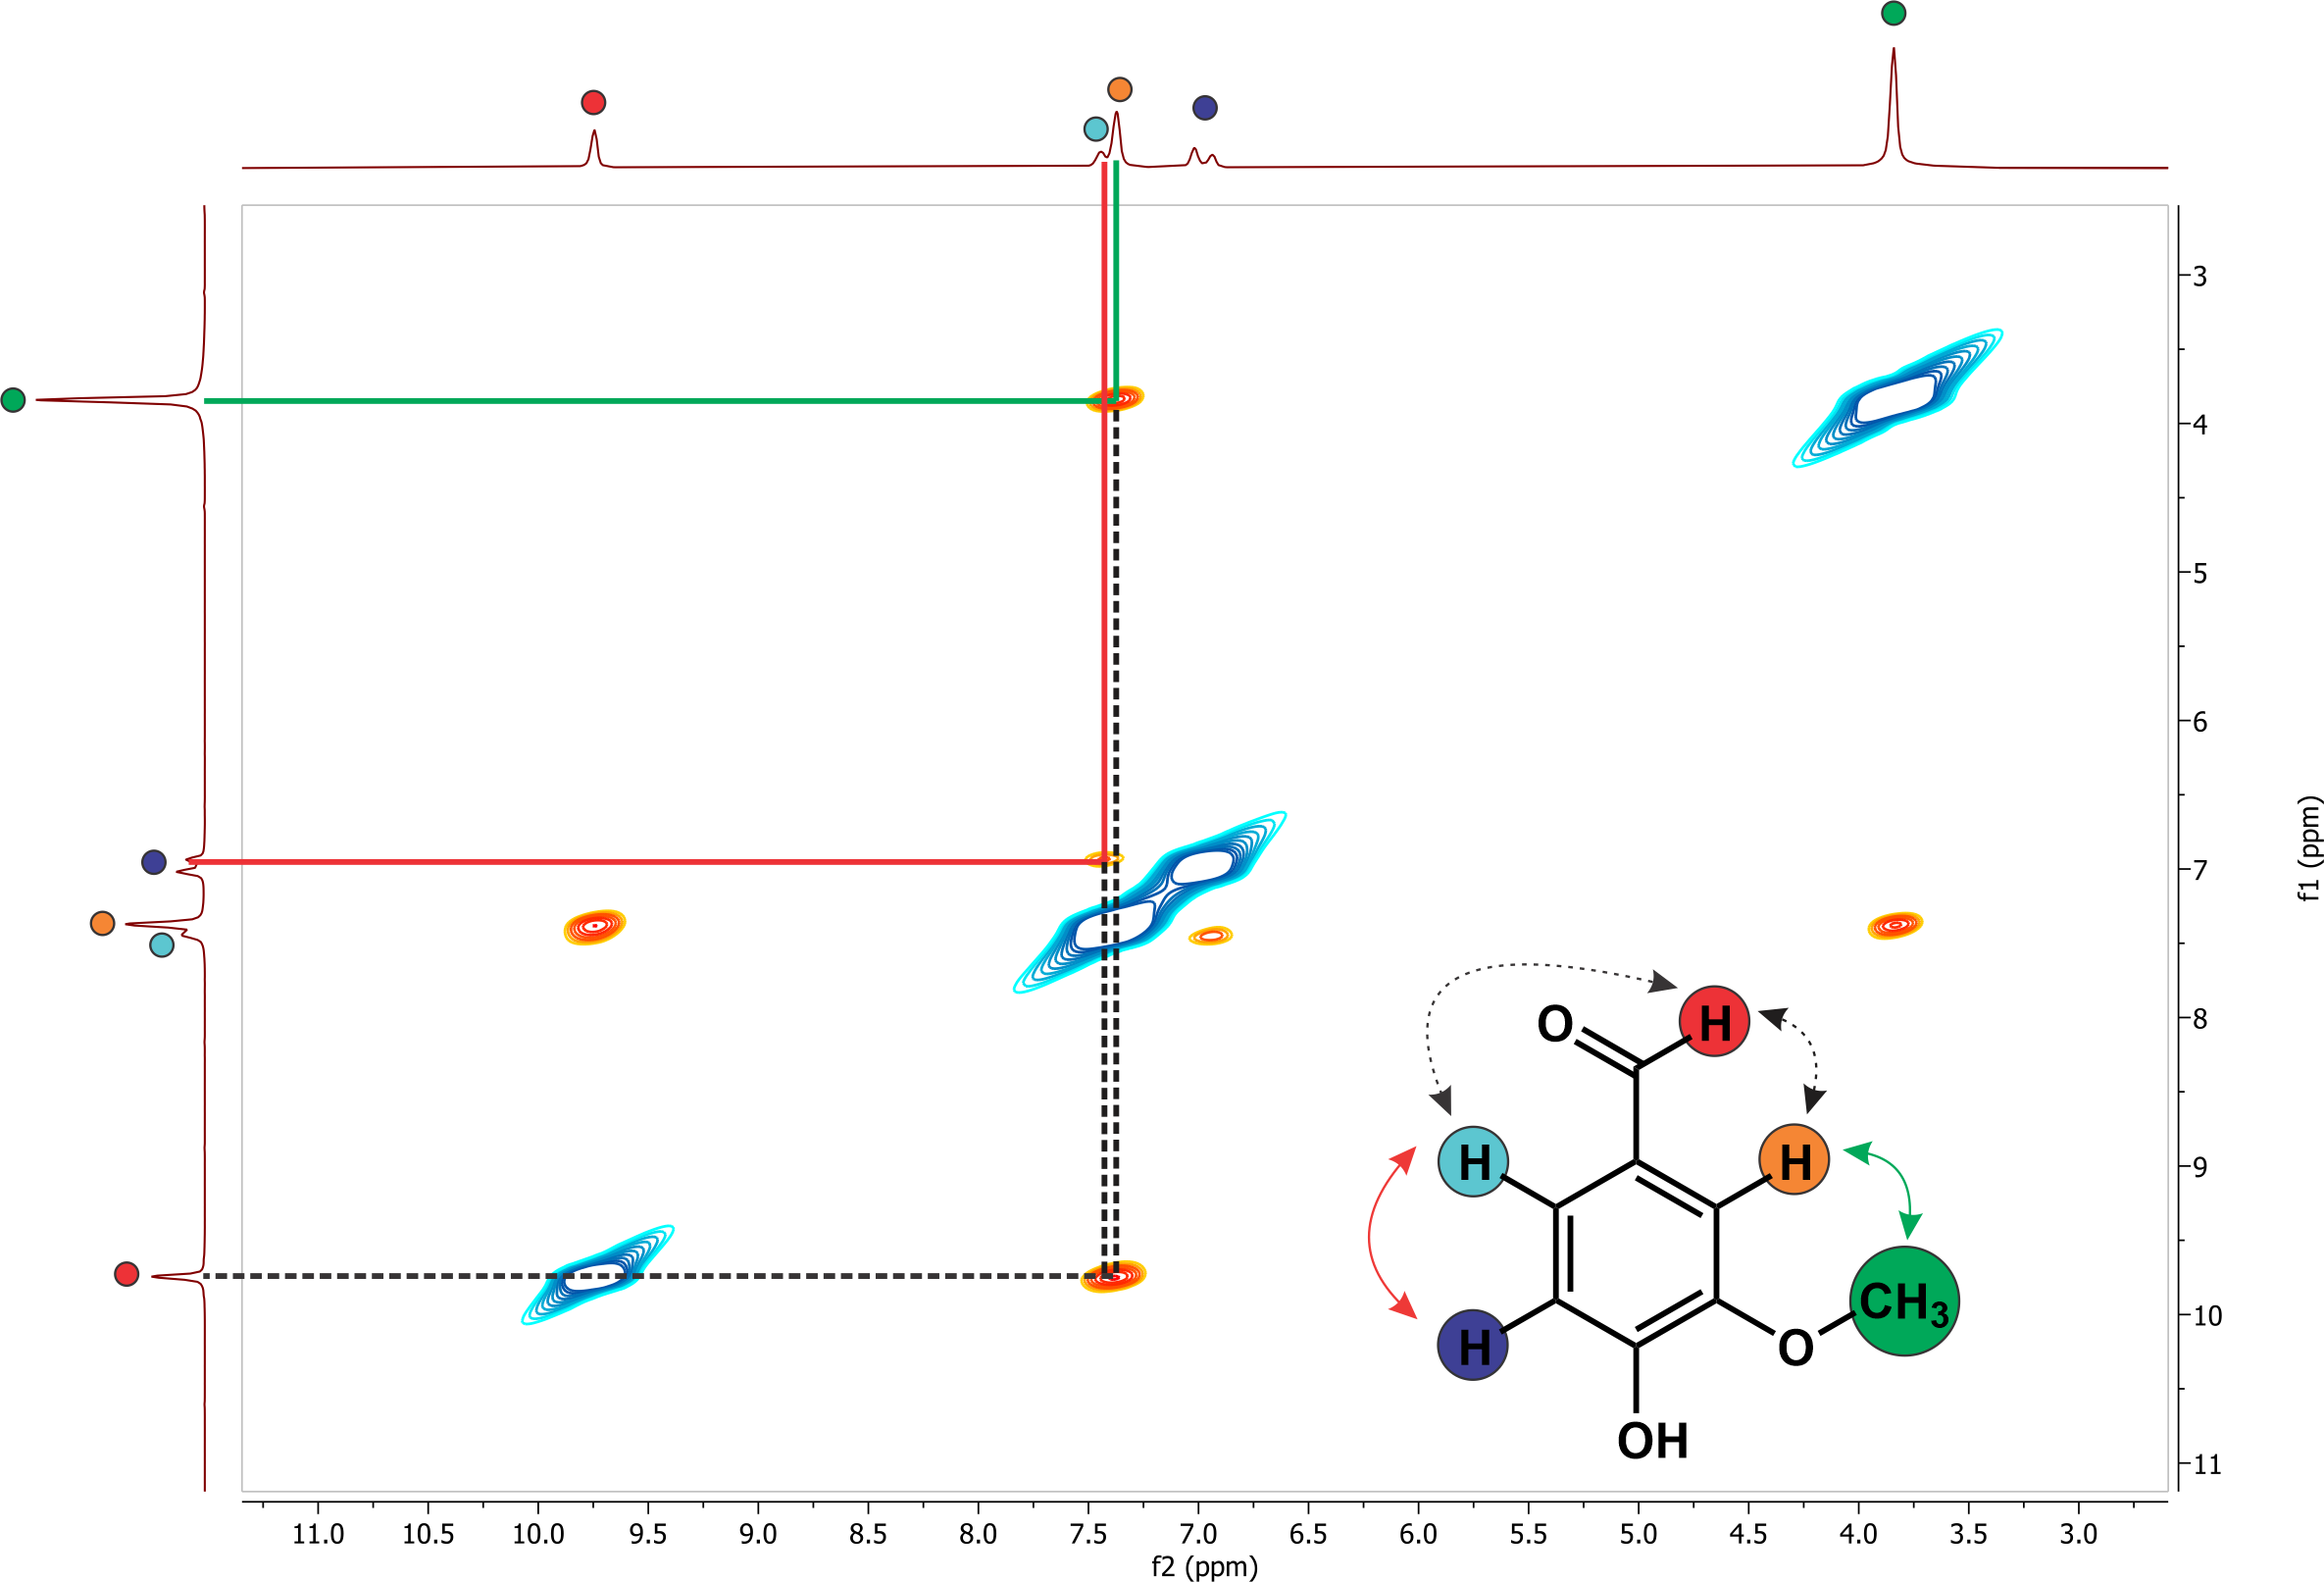
\includegraphics[width=0.8\linewidth]{NOESY.png}
        \caption{Example NOESY spectrum.}
        \label{fig:NOESY}
    \end{figure}
    \begin{itemize}
        \item This is a 2D experiment.
        \item We have two identical \ce{{}^1H} NMR experiments on the top and left sides of Figure \ref{fig:NOESY}. All of the peaks are labeled by the hydrogen(s) to which they correspond.
        \item The diagonal peaks occur at the intersection of identical peaks from the two constitutent proton NMR spectra.
        \item The 2D part comes from the off-diagonal dots. These appear at the intersection of peaks corresponding to hydrogens that couple. For example, the green interaction connects the green and orange protons, and the orange point in the plot indicates that the green and orange protons couple semi-strongly.
    \end{itemize}
    \item DEPT?
    \begin{itemize}
        \item Takeaway for DEPT: We can do 2D NMR experiments where we manipulate two spins at the same time and pull out data on both.
    \end{itemize}
    \item What do I need to know about the literature examples for the final?
    \item Question 2.1: How does an amide have $C_{2v}$ symmetry, not $C_s$ symmetry?
    \item Question 2.2.
    \begin{itemize}
        \item There are two states to consider: The ground state, which is a singlet and thus EPR silent, and the excited state, which is a triplet and thus EPR active.
    \end{itemize}
    \item Question 2.3.
    \begin{itemize}
        \item We have two main signals: A triplet of doublets centered at $-1444.85$, and a triplet of quartets centered at $1505.7$. How is this possible?
        \item Calculating nuclear spin? How would we know that \ce{Pt} has an $I=1/2$ nucleus with 33\% abundance? We can google this stuff for the pset; we won't have to just know this stuff for the test.
        \item We can ask questions about specific nuclei during the exam, but the data should be stated in the question.
        \item How do we know when \ce{P-Pt} and \ce{P-P} coupling are present?
        \item Largest magnitude coupling is usually the shortest coupling.
        \item We split based on percent abundance. Even in carbon, where you have 1\% abundance of \ce{{}^13C}, that gives rise to tiny splittings off the main peak.
        \item Essentially, here, we have an $I=0$ \ce{Pt} nucleus in 66\% abundance and an $I=1/2$ \ce{Pt} nucleus in 33\% abundance. Thus, for every phosphorous, the primary splitting modality will be to form a singlet overlaid with a doublet. Twice as many molecules will have an $I=0$ nucleus as otherwise, so this accounts for the large central peaks. Additionally, $I=1/2$ will split the doublet to $1/4$ the height of the $I=0$ peak. Then, secondary splitting occurs from the neighboring phosphorus spin centers, which are $I=1/2$ nuclei, themselves.
    \end{itemize}
    \item Question 2.4?
    \begin{itemize}
        \item Isn't square planar always low spin?
        \item It's almost exclusively low spin; you can have some weird constrained cases, though.
        \item Anderson showed the high-spin case purely for completeness and because he would have accepted the answer, but a sole low-spin answer is perfectly acceptable.
    \end{itemize}
    \item Question 2.7?
    \begin{itemize}
        \item How would isomers affect the Mossbauer spectrum?
    \end{itemize}
    \item Question 2.8?
    \begin{itemize}
        \item What is the significance of the mass number and change on \ce{{}^63Cu^2+}? Just gives you nice data.
        \item Why is $g$ isotropic in the center? Just because this is peak splitting? And isn't it isotropic anyway since it's in solution?
    \end{itemize}
    \item Question 2.9b?
    \begin{itemize}
        \item How do we get the final number?
        \item Convert the Bohr magneton to hertz; any such values will be given on the test.
        \item $\beta=\SI{1.4e10}{\per\second\per\tesla}$. Again, take $\beta/h$.
    \end{itemize}
    \item Question 2.10a?
    \begin{itemize}
        \item Could you not look for the presence of all three $K$-edges? Is it better to look at one $K$-edge and fit scatterers?
    \end{itemize}
    \item Question 2.10b?
    \begin{itemize}
        \item Generally very confused.
    \end{itemize}
    \item Question 11?
    \begin{itemize}
        \item Walk me through this.
        \item Orthogonality in all its shapes --- be it of orbital fillings, literal orbital configuration and molecular structure, bond angles, etc. --- favors FM interactions.
        \item When it goes away, AF dominates. But where is the antiparallel AF interaction with high overlap in the second case?
    \end{itemize}
    \item How will the final relate to the pset?
\end{itemize}



\section{Final Exam Review Sheet}
\begin{itemize}
    \item \marginnote{3/6:}Review character tables and that stuff!
    \item Isotope effects in IR spectroscopy.
    \begin{equation*}
        \frac{\nu_{\ce{AA}}}{\nu_{\ce{BB}}} = \frac{\sqrt{\mu_{\ce{BB}}}}{\sqrt{\mu_{\ce{AA}}}}
    \end{equation*}
    \item Basic magnetism relations and definitions.
    \begin{align*}
        B &= \frac{F}{Qv}&
        B &= \vec{H}+4\pi\vec{M}&
        \vec{f} &= \vec{M}\cdot\dv{H}{z}&
        \chi_V = \chi &= \frac{\vec{M}}{\vec{H}}&
        \chi_g &= \frac{\chi_V}{d}&
        \chi_m &= \chi_g\cdot\text{MW}
    \end{align*}
    \item Presence or absence of unpaired electrons.
    \begin{itemize}
        \item Unpaired: $\chi>0$.
        \item Paired: $\chi<0$.
    \end{itemize}
    \item Diamagnet: $S=0$.
    \item Calculating $\chi_\text{dia}$.
    \begin{equation*}
        \chi_\text{dia} = \sum\lambda+\sum n_i\chi_i
    \end{equation*}
    \item Bohr magneton; memorize value!
    \begin{equation*}
        \mB = \beta = \SI[per-mode=symbol]{9.3e-24}{\joule\per\tesla}
    \end{equation*}
    \item Calculating magnetic parameters.
    \begin{align*}
        g &\approx 2&
        \mu_\text{eff} &= \sqrt{g^2(S(S+1))}&
        \chi T &= \frac{g^2}{8}S(S+1)
    \end{align*}
    \item Spin-orbit coupling.
    \begin{itemize}
        \item $>$ half-filled shell: $g>0$.
        \item $<$ half-filled shell: $g<0$.
    \end{itemize}
    \item The magnetic coupling constant $J$.
    \begin{itemize}
        \item AM vs. FM.
        \begin{itemize}
            \item FM: $J>0$.
            \item AF: $J<0$.
        \end{itemize}
        \item Total coupling.
        \begin{equation*}
            J_\text{tot} \approx 2K+4\beta S
        \end{equation*}
        \item Maximizing the types.
        \begin{itemize}
            \item Maximizing FM: Close distance and no overlap (picture the lack of splitting in an orbital diagram enabling easy excitation). Anything more perpendicular/orthogonal, be it physical structure (\ang{90} vs. \ang{180}), orbital planes ($xy$ vs. $z$), orbital wavefunction ($\sigma$ vs. $\pi$), orbital orthogonality (different fillings of paired vs. unpaired).
            \item Maximizing AF: Long distance and big overlap (picture the large splitting in an orbital diagram forcing pairing). Anything more aligned.
        \end{itemize}
    \end{itemize}
    \item $M_\text{sat}$, $M_\text{rem}$, and $H_C$. Soft vs. hard ferromagnets.
    \item EPR energy gap.
    \begin{equation*}
        h\nu = \Delta E = g\beta H
        \quad\Longleftrightarrow\quad
        g = \frac{h\nu}{\beta H_r}
    \end{equation*}
    \item EPR graphs: Plot the first derivative of absorbance vs. magnetism.
    \item EPR $d$-values.
    \begin{itemize}
        \item $d$-orbital $<$ half-filled: $g<2$.
        \item $d$-orbital $=$ half-filled: $g\approx 2$.
        \item $d$-orbital $>$ half-filled: $g>2$.
        \item Rationalize with ring currents reinforcing $H_r$.
    \end{itemize}
    \item EPR hyperfine Zeeman splitting.
    \begin{itemize}
        \item Caused by coupling to the nucleus.
        \item Selection rules.
        \begin{align*}
            \Delta M_I &= 0&
            \Delta M_S &= \pm 1
        \end{align*}
        \item $a$ is the actual hyperfine coupling constant in Joules; $A$ is the measured hyperfine coupling constant in Teslas.
        \begin{equation*}
            a = g\beta A
        \end{equation*}
        \item $M_I$ sums from neighboring nuclei with no preference.
        \item Number of peaks.
        \begin{equation*}
            2nI+1
        \end{equation*}
    \end{itemize}
    \item ENDOR selection rules.
    \begin{align*}
        \Delta M_S &= \pm 1&
        \Delta M_I &= \pm 1
    \end{align*}
    \item XAS: Pre-edge, edge, XANES, EXAFS.
    \item $K$-edge: $n=1$ electron.
    \item $L$-edge: $n=2$ electron.
    \item Pre-edge: Symmetry information; symmetry decreases $\Rightarrow$ more coupling $\Rightarrow$ pre-edge increases.
    \item $K$-edge: Oxidation state.
    \item EXAFS.
    \begin{itemize}
        \item Number, type, and distance of scatters.
        \item Heavier atoms scatter more.
    \end{itemize}
    \item Mossbauer: Gamma rays excite nuclei.
    \begin{equation*}
        E_\gamma = E_R+D-R
    \end{equation*}
    \item Electron density at nucleus; isomer shift; higher oxidation state $\Rightarrow$ less electron density $\Rightarrow$ lower isomer shift.
    \item Electronic symmetry; The greater the asymmetry, the higher $\Delta E_Q$.
    \begin{equation*}
        \Delta = e^2qQ
    \end{equation*}
    \item Magnetic field: Nuclear levels split.
    \item EChem.
    \item Nernst equation.
    \begin{equation*}
        E_\text{app} = E^\circ+\frac{RT}{nF}\ln\frac{[\text{Ox}]}{[\text{Red}]}
    \end{equation*}
    \item NMR.
    \item Energy difference.
    \begin{equation*}
        \Delta E = \gamma\hbar B_0
    \end{equation*}
    \item Larmor frequency.
    \begin{equation*}
        \nu_0 = \frac{\gamma B_0}{2\pi}
    \end{equation*}
    \item Chemical shift.
    \begin{equation*}
        \SI{1}{\ppm} = \frac{\nu_1-\nu_\text{ref}}{\nu_0}\times\num{e6}
    \end{equation*}
    \item Chemical shift lingo.
    \begin{itemize}
        \item More \emph{shielded} nuclei require \emph{higher fields}, resonate at \emph{lower frequencies}, have a \emph{lower chemical shift}, and are positioned relatively \emph{upfield} (to the \emph{right} on a spectrum).
        \item More \emph{deshielded} nuclei resonate at \emph{lower fields}, require \emph{higher frequencies}, have a \emph{higher chemical shift}, and are positioned relatively \emph{downfield} (to the \emph{left} on a spectrum).
    \end{itemize}
    \item The actual coupling constant is $J$.
    \begin{itemize}
        \item Single bond: $J>0$, antiparallel spins.
        \item Double dond: $J<0$, parallel spins.
        \item Hybridization decreases: $J$ increases (things are held tighter).
        \item Electronegativity decreases: $J$ decreases (things get more $s$-character, so less is available for coupling).
        \item $J_\text{trans}>J_\text{cis}$.
        \item $J_\text{syn}\approx J_\text{anti}>J_\text{gauche}$.
        \item $J_\text{trans}>J_\text{cis}>J_\text{gem}$.
    \end{itemize}
    \item Hahn echo pulses and decays.
    \item NOE enhanced for closer protons.
\end{itemize}




\end{document}